\section{Android Application for SSPS Demo}

The Android application demonstrates the SSPS for mobile applications by showing the throughput comparison with and without the use of SSPS. The application will provide the provision to subscribe to a set of topics. Each topic would correspond to messages being received by the Android application in different formats such as JSON, XML, and CSV. The messages would contain location coordinates which will be displayed on a map. 

\subsection{Architecture}

Figure \ref{figures:android} depicts the architecture of the system that is used to demonstrate the SSPS for mobile applications. There are three publishers named XML, CSV and JSON, which publish the same data in XML, CSV, and JSON format respectively. All the publishers publish both compressed messages using the dictionaries received from the sampling broker and also plain uncompressed messages for the same data format, for, e.g., XML publisher publishes both compressed and uncompressed messages in XML format. The Android application initially connects to the sampling broker and receive the dictionaries. Once the application has connected to the sampling broker, it receives the messages. The application has controls to subscribe to topics which enable it to receive messages corresponding to any data format (XML, CSV, and JSON) and type (compressed or uncompressed).
At any instant, the application receives data from only one topic.

\makeatletter
\setlength{\intextsep}{20pt}
\makeatother

\begin{figure}[h!]
\centering
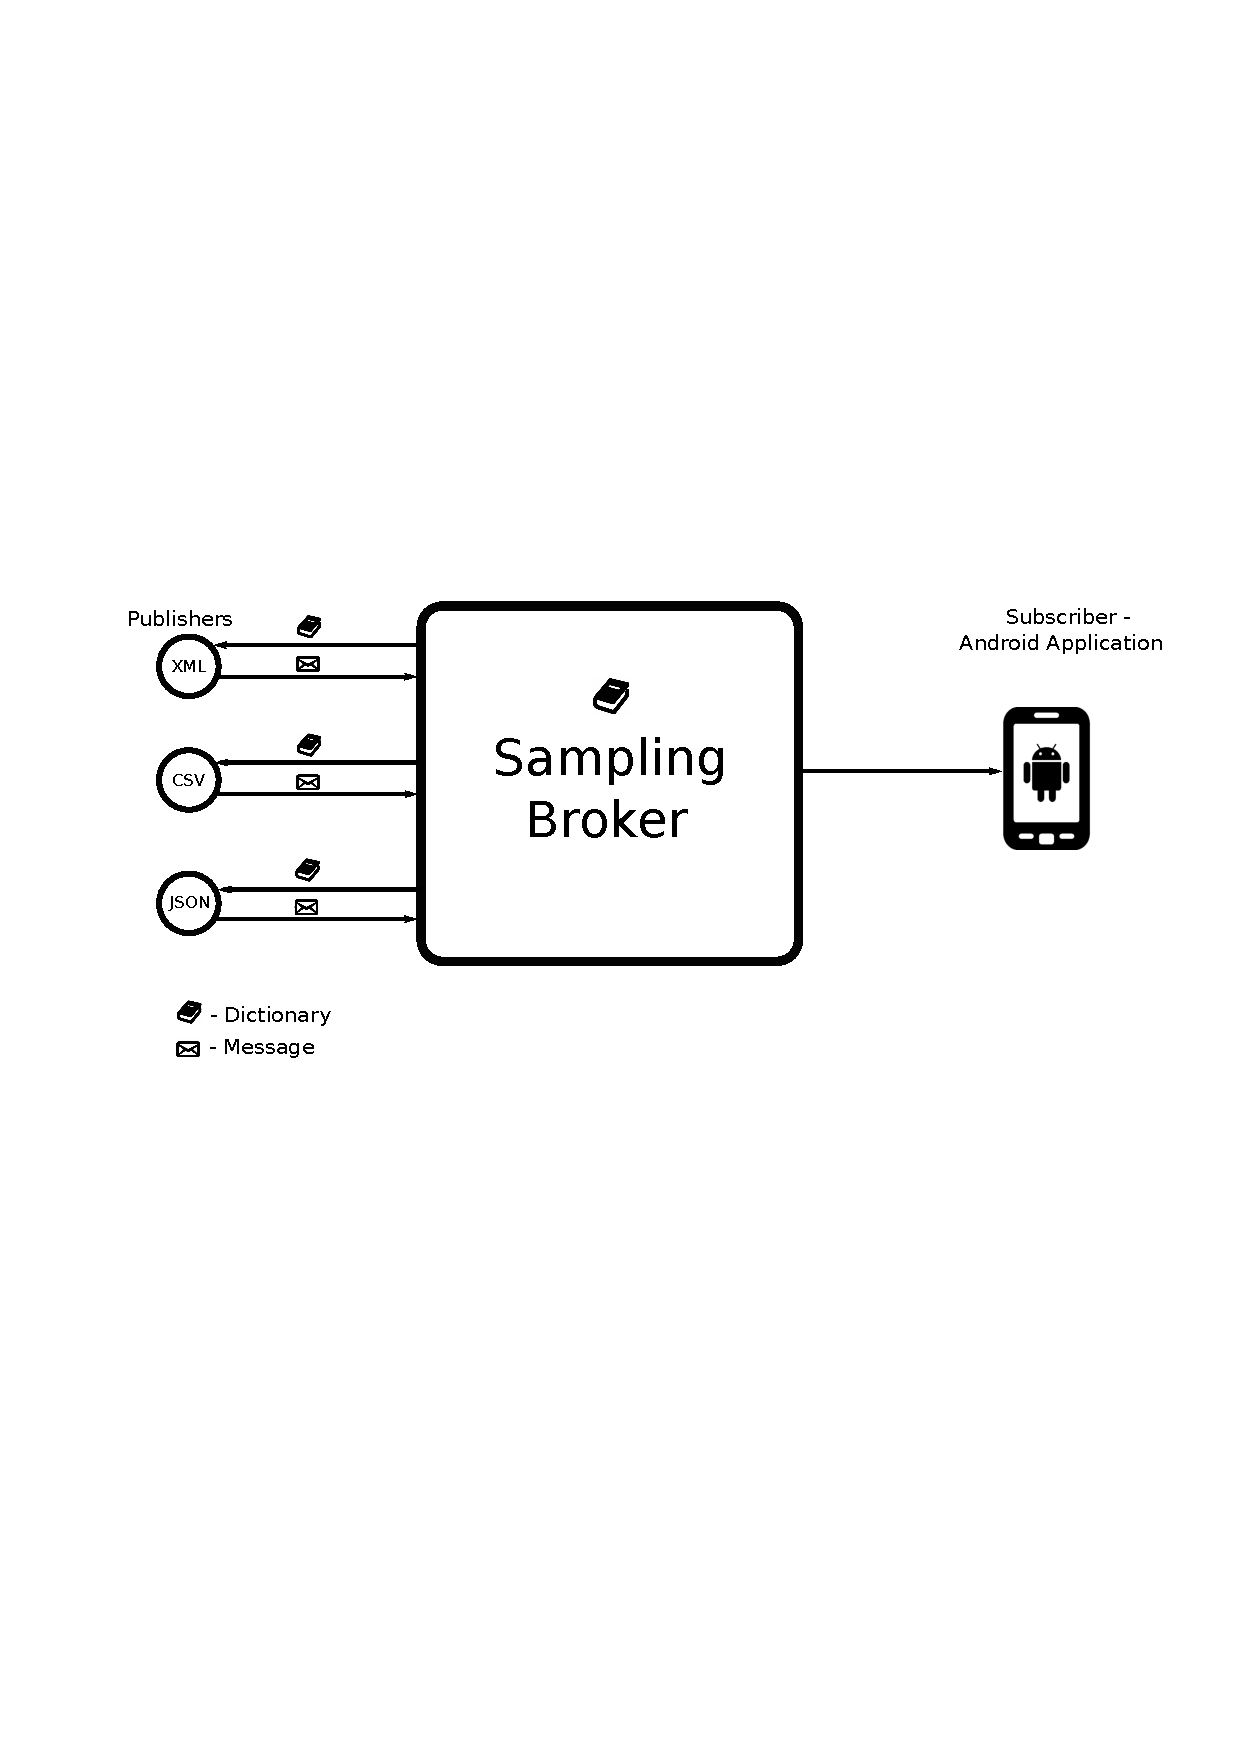
\includegraphics[keepaspectratio, width=1.0\textwidth, trim={0 11cm 0 9cm},clip]{android.pdf}
\caption{Architecture for SSPS demonstration}\label{figures:android}
\end{figure}

\subsection{UI Design}

Figure \ref{figures:android_ui} depicts the UI design of the Android application. The components are described below.

\makeatletter
\setlength{\intextsep}{20pt}
\makeatother

\begin{figure}[h!]
\centering
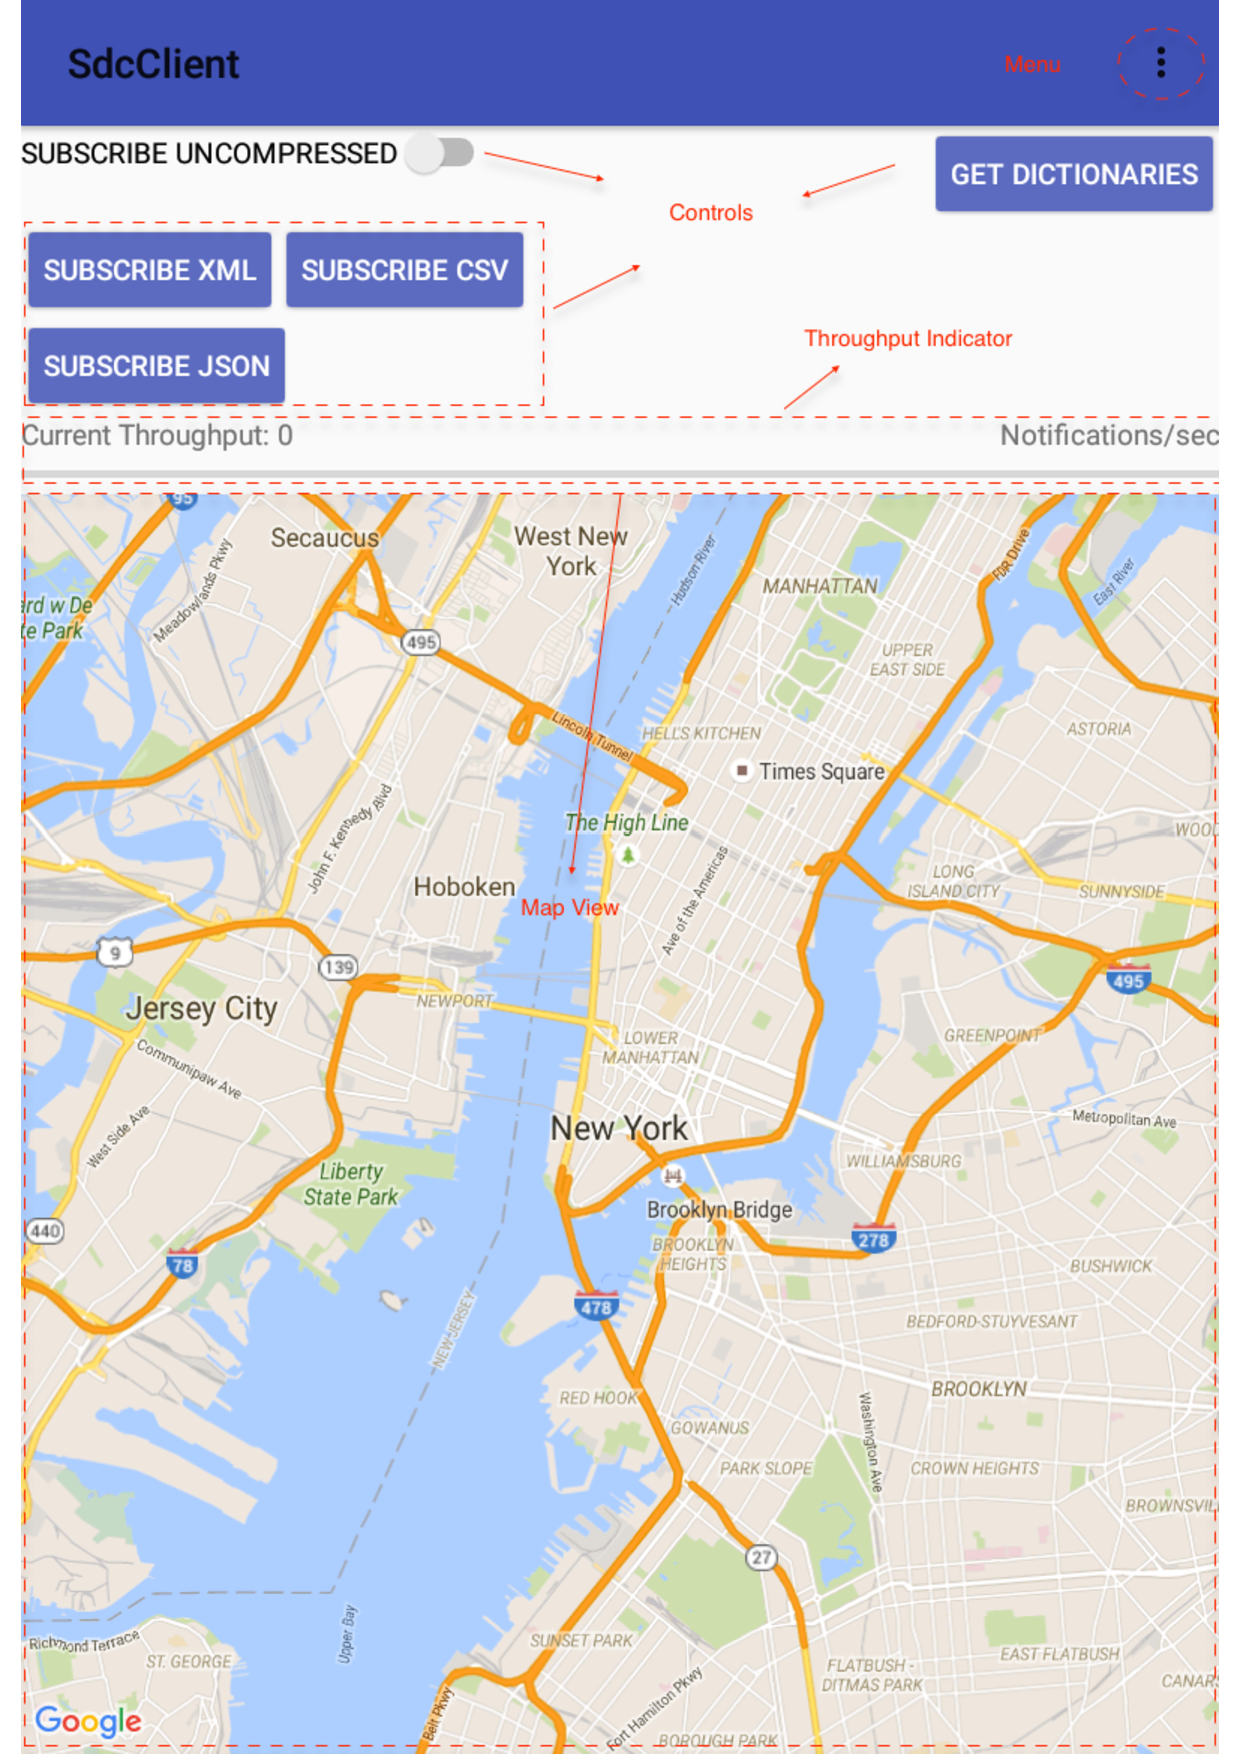
\includegraphics[keepaspectratio, width=0.85\textwidth, trim={0 0 0 0},clip]{android_ui.pdf}
\caption{Android Application UI Design for SSPS}\label{figures:android_ui}
\end{figure}

\begin{itemize}
    \item \textbf{Menu:}
          It contains two options: 
            \begin{itemize}
                \item \textbf{Enter IP:}
                Presents a dialog box to enter IP address for connecting to the sampling broker.
                \item \textbf{Stop:}
                Stops the application by disconnecting from the sampling broker.
            \end{itemize}

    \item \textbf{Controls:}
    Controls consist of four buttons and a switch.
    \begin{itemize}
        \item \textbf{GET DICTIONARIES:}
        This button enables to get all the required dictionaries upfront since sampling of the dictionaries takes time.
        \item \textbf{SUBSCRIBE XML:}
        This button enables to subscribe to the XML topic.
        \item \textbf{SUBSCRIBE CSV:}
        This button enables to subscribe to the CSV topic.
        \item \textbf{SUBSCRIBE JSON:}
        This button enables to subscribe to the JSON topic.
        \item \textbf{SUBSCRIBE UNCOMPRESSED:}
        This switch enables to toggle between the subscription of compressed and uncompressed version of the currently active subscription.
    \end{itemize}

    \item \textbf{Throughput indicator and Map View:}
    These are explained in detail in the subsequent sections.
\end{itemize}

\subsection{Throughput Indicator}

The throughput indicator indicates the current throughput in terms of number of notifications received per second. It shows a numeric value of the current throughput and also indicates on a progress bar.

\makeatletter
\setlength{\intextsep}{20pt}
\makeatother

\begin{figure}[h!]
\centering
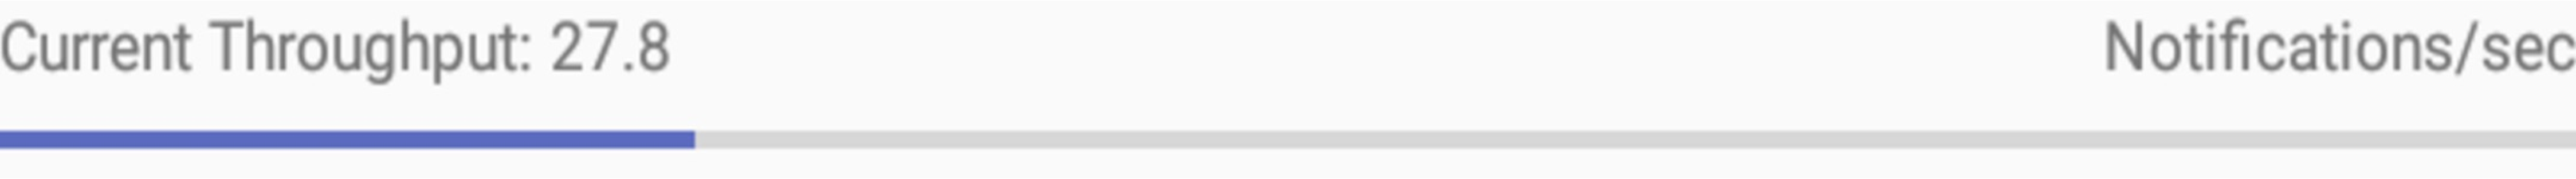
\includegraphics[keepaspectratio, width=0.85\textwidth, trim={0 0 0 0},clip]{throughput.pdf}
\caption{Android Application Throughput Indicator}\label{figures:android_throughput}
\end{figure}

Figure {\ref{figures:android_throughput}} depicts the throughput indicator indicating a throughput of 27.8 Notifications/sec. This is also represented by a blue line below the numeric throughput.

\subsubsection{Calculation}

The throughput calculation in the Android application is the weighted average of last five throughput values.
Listing \ref{lst:code_throughput} shows the code snippet used for the calculating the weighted throughput.

\bigskip
\begin{lstlisting}[style=JavaInputStyle,caption=Throughput calculation code snippet, label={lst:code_throughput}]

    for (float v : throughputValues)
        val += v;
    final float weightedThroughput = val / 5;

    MainActivity.this.runOnUiThread(new Runnable() {
        @Override
        public void run() {
            publishThroughput(weightedThroughput);
        }
    });
    throughputValues.remove(0);

\end{lstlisting}

\subsection{Map View}

The map view indicates the arrival of notifications. The dataset (explained in a later section) used for the demonstration, has a location co-ordinates as part of every message. We show this location coordinates on the map.  

\makeatletter
\setlength{\intextsep}{20pt}
\makeatother

\begin{figure}[h!]
\centering
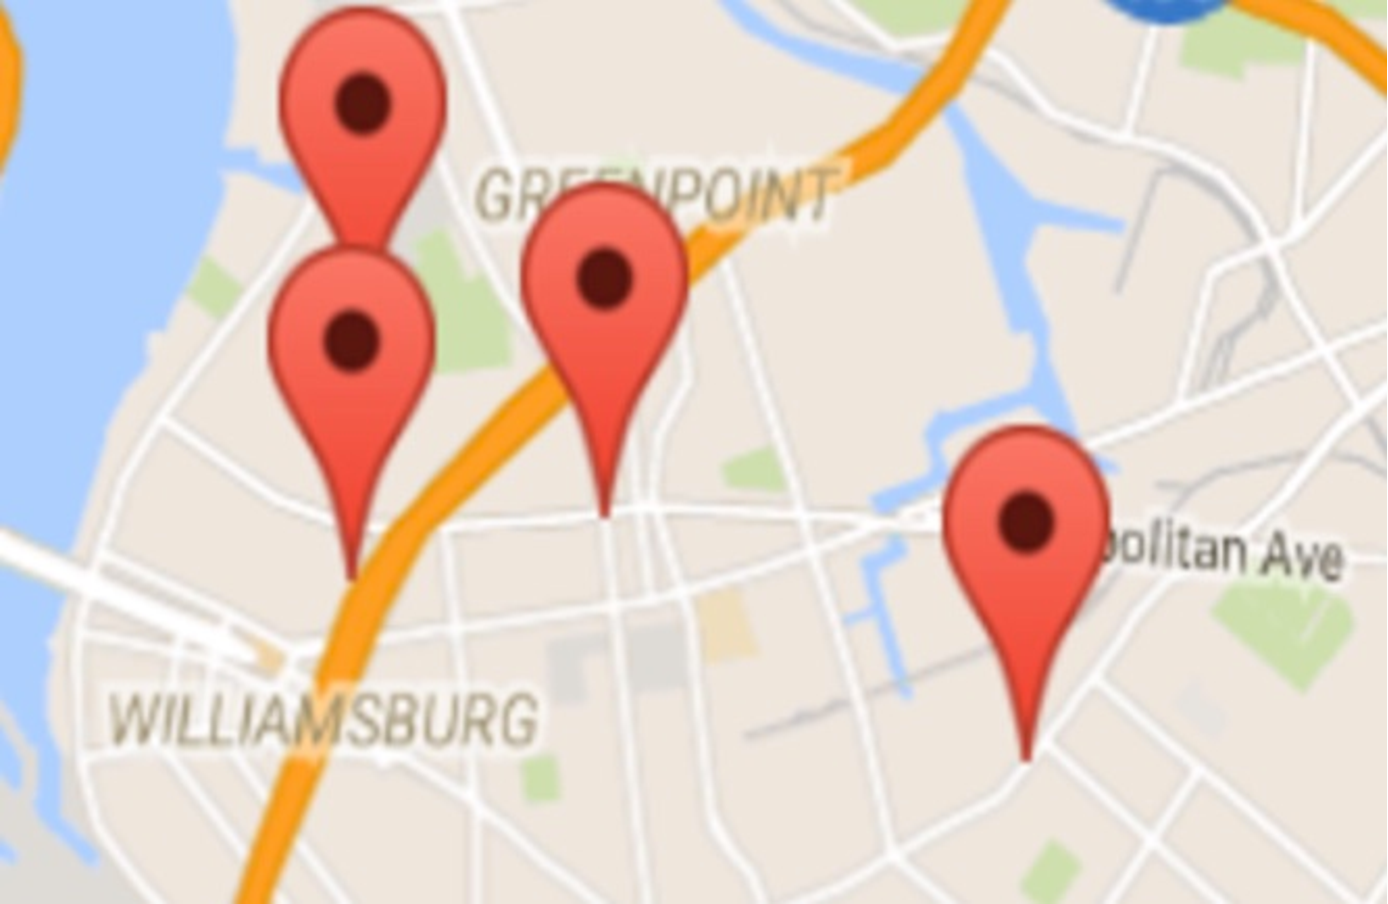
\includegraphics[keepaspectratio, width=0.5\textwidth, trim={0 0 0 0},clip]{mapview.pdf}
\caption{Android Application Map View}\label{figures:android_map}
\end{figure}

Figure \ref{figures:android_map} depicts a part of the map view with four notifications indicated by four markers. To avoid cluttering on the map with many markers, we display on the last one hundred markers indicating last one hundred notifications.

Listing \ref{lst:code_marker} shows the function that adds a marker on the map view corresponding to every notification received by the Android application.

\bigskip
\begin{lstlisting}[style=JavaInputStyle,caption=Function to add marker on Map, label={lst:code_marker}]

    private void publishCoordinates(String latitude, String longitude) {
        LatLng location = new LatLng(Double.parseDouble(latitude), Double.parseDouble(longitude));
        Marker marker = mMap.addMarker(new MarkerOptions().position(location));
        markers.add(marker);
        if (markers.size() == 100) {
            markers.get(0).setVisible(false);
            markers.remove(0);
        }
    }

\end{lstlisting}